%% ----------------------------------------------------------------------------
%%  §11.6  Criteri di convergenza per le serie a termini non negativi
%% ----------------------------------------------------------------------------
\section{Criteri di convergenza}
\label{sec:criteri-convergenza}

Calcolare esplicitamente la somma di una serie è possibile solo in pochi casi (le
serie geometriche, le telescopiche, poche altre); per questo, nelle applicazioni, la somma
si calcola spesso numericamente. Prima di farlo, però, occorre sapere se la serie
converge: sommare con un calcolatore il primo milione di termini della serie armonica
darebbe circa $14{,}4$, un numero del tutto privo di significato come «somma». I \emph{criteri di
convergenza} stabiliscono il carattere di una serie senza calcolarne la somma. In tutto
questo paragrafo consideriamo serie \emph{a termini non negativi}, che per il
\cref{teo:serie-positive} sono convergenti o divergenti a $+\infty$. Per il teorema del resto
(\cref{teo:resto-serie}) basta che le ipotesi siano verificate da un certo indice in poi.

\subsection{Il criterio del confronto}

\begin{teorema}[Criterio del confronto]\label{teo:confronto-serie}
\index{criterio del confronto!per le serie}
Siano $a_{n}$ e $b_{n}$ due successioni tali che $0\le a_{n}\le b_{n}$ per ogni $n$. Allora
\begin{align}
  \sum_{k=1}^{\infty}b_{k}<+\infty &\implica \sum_{k=1}^{\infty}a_{k}<+\infty ; \label{eq:confronto-conv}\\
  \sum_{k=1}^{\infty}a_{k}=+\infty &\implica \sum_{k=1}^{\infty}b_{k}=+\infty . \label{eq:confronto-div}
\end{align}
\end{teorema}

\begin{schema}
\Ipotesi{$0\le a_{n}\le b_{n}$ per ogni $n$ (o per ogni $n>\nu$).}
\Tesi{se converge la serie maggiorante $\sum b_{k}$, converge la minorante $\sum a_{k}$; se
diverge la minorante, diverge la maggiorante.}
\end{schema}

\begin{strategia}
Le somme parziali $s_{n}$ di $\sum a_{k}$ e $t_{n}$ di $\sum b_{k}$ verificano $s_{n}\le t_{n}$, e hanno
entrambe limite perché le serie sono a termini non negativi. Basta allora confrontare i
limiti.
\end{strategia}

\begin{dimostrazione}
Siano $s_{n}=\sum_{k=1}^{n}a_{k}$ e $t_{n}=\sum_{k=1}^{n}b_{k}$. Dall'ipotesi segue $s_{n}\le t_{n}$ per ogni $n$,
e per il \cref{teo:serie-positive} entrambe le successioni hanno limite. Se
$\lim t_{n}=t<+\infty$, allora $s_{n}\le t_{n}\le t$ per ogni $n$ (una successione crescente non
supera il proprio limite), e $s_{n}$, crescente e limitata, converge: vale la
\eqref{eq:confronto-conv}. Se invece $s_{n}\to+\infty$, da $t_{n}\ge s_{n}$ e dal teorema del
confronto (\cref{teo:confronto-infinito}) segue $t_{n}\to+\infty$: vale la
\eqref{eq:confronto-div}. Se l'ipotesi vale solo per $n>\nu$, si applica quanto detto ai
resti $\nu$-esimi e si conclude con il \cref{teo:resto-serie}.
\end{dimostrazione}

\begin{esempio}\label{es:confronto}
\begin{enumerate}[label=(\alph*)]
  \item $\sum\frac1{k^{2}+k+1}$ converge, perché $0<\frac1{k^{2}+k+1}<\frac1{k^{2}}$ e $\sum\frac1{k^{2}}<+\infty$.
  \item $\sum\frac{\sen^{2}k}{k^{2}}$ converge, perché $0\le\frac{\sen^{2}k}{k^{2}}\le\frac1{k^{2}}$.
  \item $\sum\frac{\log k}k$ diverge, perché $\frac{\log k}k\ge\frac1k$ per $k\ge3$ (essendo $\log k\ge1$
  per $k\ge e$) e la serie armonica diverge.
\end{enumerate}
\end{esempio}

\subsection{Il criterio degli infinitesimi e il confronto asintotico}

Spesso il termine generale non è maggiorato da quello di una serie nota, ma è
«dello stesso ordine» di $\frac1{n^{p}}$. Trasportiamo alle successioni il linguaggio degli
infinitesimi introdotto per le funzioni (\cref{def:parte-principale}): due successioni
$a_{n}$ e $b_{n}>0$ si dicono \emph{equivalenti}, e si scrive $a_{n}\sim b_{n}$, se $\frac{a_{n}}{b_{n}}\to1$; se
$n^{p}a_{n}\to\ell\in(0,+\infty)$ per un numero reale $p>0$, si dice che $a_{n}$ è un \emph{infinitesimo di
ordine $p$} (rispetto a $\frac1n$) con \emph{parte principale} $\frac\ell{n^{p}}$, e si ha $a_{n}\sim\frac\ell{n^{p}}$. Il
criterio seguente traduce il confronto in un limite.

\needspace{12\baselineskip}
\begin{teorema}[Criterio degli infinitesimi]\label{teo:criterio-infinitesimi}
\index{criterio degli infinitesimi}
Sia $a_{n}\ge0$ e supponiamo che, per un numero reale $p$, esista il limite
\begin{equation}\label{eq:limite-infinitesimi}
  \ell=\lim_{n\to+\infty}n^{p}a_{n}\in[0,+\infty] .
\end{equation}
Allora
\begin{align}
  \ell<+\infty,\ p>1 &\implica \sum_{k=1}^{\infty}a_{k}<+\infty ; \label{eq:infinitesimi-conv}\\
  \ell>0,\ p\le1 &\implica \sum_{k=1}^{\infty}a_{k}=+\infty . \label{eq:infinitesimi-div}
\end{align}
\end{teorema}

\begin{schema}
\Ipotesi{$a_{n}\ge0$; \ $n^{p}a_{n}\to\ell\in[0,+\infty]$.}
\Tesi{$\ell$ finito e $p>1$ $\implica$ convergenza; \ $\ell\neq0$ e $p\le1$ $\implica$ divergenza.}
\end{schema}

\begin{strategia}
Se $n^{p}a_{n}$ ha limite finito, da un certo punto in poi è minore di $\ell+1$, cioè
$a_{n}<\frac{\ell+1}{n^{p}}$: si confronta con la serie armonica generalizzata, che converge per
$p>1$. Se il limite è positivo, da un certo punto in poi $n^{p}a_{n}$ supera un numero
positivo $c$, cioè $a_{n}>\frac c{n^{p}}$, e per $p\le1$ la minorante diverge.
\end{strategia}

\begin{dimostrazione}
Sia $\ell<+\infty$ e $p>1$. Per la definizione di limite (con $\epsilon=1$) esiste $\nu$ tale che
$n^{p}a_{n}<\ell+1$ per ogni $n>\nu$, cioè $0\le a_{n}<\frac{\ell+1}{n^{p}}$. La serie di termine generale
$\frac{\ell+1}{n^{p}}$ converge (\cref{teo:armonica-generalizzata,prop:linearita-serie}), e per il
criterio del confronto converge anche $\sum a_{k}$.

Sia $\ell>0$ e $p\le1$. Scegliamo un numero $c$ con $0<c<\ell$ (ad esempio $c=\frac\ell2$ se
$\ell$ è finito, $c=1$ se $\ell=+\infty$). Poiché $n^{p}a_{n}-c$ ha limite positivo (o $+\infty$),
per la permanenza del segno esiste $\nu$ tale che $n^{p}a_{n}>c$ per $n>\nu$, cioè $a_{n}>\frac c{n^{p}}$. La serie di
termine generale $\frac c{n^{p}}$ diverge, e per il criterio del confronto diverge anche
$\sum a_{k}$.
\end{dimostrazione}

Il criterio non decide quando $\ell=0$ e $p\le1$, oppure $\ell=+\infty$ e $p>1$. Ad esempio, per
$a_{n}=\frac1{n\log n}$ si ha $na_{n}\to0$ e $n^{p}a_{n}\to+\infty$ per ogni $p>1$: il criterio degli
infinitesimi tace. Il criterio dell'integrale, invece, decide (la sua dimostrazione vale
senza modifiche per una funzione continua, non negativa e decrescente su $[k_{0},+\infty)$, con
le somme che partono da $k_{0}$): con $f(x)=\frac1{x\log x}$, decrescente per $x\ge2$, si ha $\int_{2}^{b}\frac{dx}{x\log x}=\log\log b-\log\log2\to+\infty$, e la serie
$\sum_{k=2}^{\infty}\frac1{k\log k}$ diverge, ancora più lentamente della serie armonica. Allo stesso
risultato conduce, senza integrali, il criterio di condensazione
(\cref{es:condensazione-log}).

Quando il limite \eqref{eq:limite-infinitesimi} è finito e positivo, cioè quando $a_{n}$ è un
infinitesimo di ordine $p$ con parte principale $\frac\ell{n^{p}}$, la serie converge se e solo
se $p>1$. È un caso particolare di un principio generale.

\begin{corollario}[Confronto asintotico]\label{cor:confronto-asintotico}
\index{criterio del confronto!asintotico}
Siano $a_{n}\ge0$ e $b_{n}>0$, con $\frac{a_{n}}{b_{n}}\to L$, dove $0<L<+\infty$. Allora le serie
$\sum a_{k}$ e $\sum b_{k}$ hanno lo stesso carattere. In particolare, se $a_{n}\sim b_{n}$ le due serie
convergono o divergono insieme.
\end{corollario}

\begin{schema}
\Ipotesi{$a_{n}\ge0$, $b_{n}>0$; \ $\frac{a_{n}}{b_{n}}\to L\in(0,+\infty)$.}
\Tesi{$\sum a_{k}<+\infty\ \sse\ \sum b_{k}<+\infty$.}
\end{schema}

\begin{strategia}
Se il rapporto tende a un numero positivo e finito, da un certo punto in poi è compreso
tra due costanti positive, ad esempio $\frac L2$ e $\frac{3L}2$: ciascuna delle due successioni è
allora maggiorata da un multiplo dell'altra, e il criterio del confronto si applica
nelle due direzioni.
\end{strategia}

\begin{dimostrazione}
Per la definizione di limite, con $\epsilon=\frac L2$, esiste $\nu$ tale che
$\frac L2<\frac{a_{n}}{b_{n}}<\frac{3L}2$, cioè $\frac L2\,b_{n}<a_{n}<\frac{3L}2\,b_{n}$, per $n>\nu$. Se $\sum b_{k}$
converge, converge $\sum\frac{3L}2b_{k}$, e quindi $\sum a_{k}$; se $\sum b_{k}$ diverge, diverge
$\sum\frac L2b_{k}$, e quindi $\sum a_{k}$. Si conclude con il criterio del confronto e il
\cref{teo:resto-serie}.
\end{dimostrazione}

\begin{esempio}\label{es:infinitesimi}
\begin{enumerate}[label=(\alph*)]
  \item La serie $\sum\frac{2k+1}{k^{5}+4k+3}$ converge: con $p=4$,
  $n^{4}\frac{2n+1}{n^{5}+4n+3}\to2$. Il termine generale «si comporta come» $\frac2{n^{4}}$.
  \item La serie $\sum\bigl(1-\cos\frac1k\bigr)$ converge: dallo sviluppo del coseno,
  $1-\cos\frac1n=\frac1{2n^{2}}+o\bigl(\frac1{n^{2}}\bigr)$, cioè $n^{2}\bigl(1-\cos\frac1n\bigr)\to\frac12$.
  \item La serie $\sum\sen\frac1k$ diverge: $n\sen\frac1n\to1$ (limite notevole), e $p=1$.
  \item La serie $\sum\bigl(\frac1k-\sen\frac1k\bigr)$ converge: per lo sviluppo del seno il termine
  generale ha parte principale $\frac1{6n^{3}}$. La differenza di due serie divergenti può
  dunque convergere.
\end{enumerate}
In tutti questi esempi lo strumento decisivo è la parte principale del termine generale,
che gli sviluppi di Taylor del \cref{cap:taylor} forniscono con poca fatica.
\end{esempio}

\subsection{I criteri del rapporto e della radice}

Gli ultimi due criteri confrontano la serie con la serie geometrica, e sono adatti
quando il termine generale contiene potenze di esponente $n$ o fattoriali.

\needspace{10\baselineskip}
\begin{teorema}[Criterio del rapporto]\label{teo:criterio-rapporto-serie}
\index{criterio del rapporto!per le serie}
Sia $a_{n}>0$ e supponiamo che esista il limite
\begin{equation}\label{eq:limite-rapporto}
  \ell=\lim_{n\to+\infty}\frac{a_{n+1}}{a_{n}} .
\end{equation}
Allora: se $\ell<1$ la serie $\sum a_{k}$ converge; se $\ell>1$ (anche $\ell=+\infty$) la serie
diverge.
\end{teorema}

\begin{schema}
\Ipotesi{$a_{n}>0$; \ $\frac{a_{n+1}}{a_{n}}\to\ell\in[0,+\infty]$.}
\Tesi{$\ell<1\implica\sum a_{k}<+\infty$; \ $\ell>1\implica\sum a_{k}=+\infty$.}
\end{schema}

\begin{strategia}
Se il rapporto tra termini consecutivi è definitivamente minore di un numero $q<1$, i
termini decrescono almeno come quelli di una progressione geometrica di ragione $q$, e la
serie si confronta con la serie geometrica convergente. Se invece il rapporto è
definitivamente maggiore di $1$, i termini crescono e non possono tendere a zero.
\end{strategia}

\begin{dimostrazione}
Sia $\ell<1$ e fissiamo $q$ con $\ell<q<1$. Per la definizione di limite (con $\epsilon=q-\ell$)
esiste $\nu$ tale che $\frac{a_{n+1}}{a_{n}}<q$ per ogni $n\ge\nu$. Allora $a_{\nu+1}<a_{\nu}q$,
$a_{\nu+2}<a_{\nu+1}q<a_{\nu}q^{2}$ e, per induzione,
\[
  a_{n}\le a_{\nu}\,q^{n-\nu}=\frac{a_{\nu}}{q^{\nu}}\,q^{n} \qquad\perogni n\ge\nu .
\]
La serie di termine generale $\frac{a_{\nu}}{q^{\nu}}q^{n}$ è una serie geometrica di ragione
$q\in(0,1)$, moltiplicata per una costante, e quindi converge; per il criterio del confronto
converge anche $\sum a_{k}$.

Sia $\ell>1$. Per la permanenza del segno esiste $\nu$ tale che $\frac{a_{n+1}}{a_{n}}>1$ per $n>\nu$:
la successione $a_{n}$ è strettamente crescente da $\nu$ in poi, e poiché $a_{n}>0$ si ha
$a_{n}>a_{\nu+1}>0$ per $n>\nu+1$. Dunque $a_{n}$ non tende a zero, e la serie diverge
(\cref{teo:condizione-necessaria,teo:serie-positive}).
\end{dimostrazione}

\begin{teorema}[Criterio della radice]\label{teo:criterio-radice}\index{criterio della radice}
Sia $a_{n}\ge0$ e supponiamo che esista il limite
\begin{equation}\label{eq:limite-radice}
  \ell=\lim_{n\to+\infty}\sqrt[n]{a_{n}} .
\end{equation}
Allora: se $\ell<1$ la serie $\sum a_{k}$ converge; se $\ell>1$ la serie diverge.
\end{teorema}

\begin{schema}
\Ipotesi{$a_{n}\ge0$; \ $\sqrt[n]{a_{n}}\to\ell\in[0,+\infty]$.}
\Tesi{$\ell<1\implica\sum a_{k}<+\infty$; \ $\ell>1\implica\sum a_{k}=+\infty$.}
\end{schema}

\begin{strategia}
Come per il criterio del rapporto, si confronta con una serie geometrica. Se
$\sqrt[n]{a_{n}}$ è definitivamente minore di un numero $q<1$, elevando alla $n$ si ottiene
$a_{n}<q^{n}$; se è definitivamente maggiore di $1$, il termine generale non tende a zero.
\end{strategia}

\begin{dimostrazione}
Sia $\ell<1$ e $q$ con $\ell<q<1$. Esiste $\nu$ tale che $\sqrt[n]{a_{n}}<q$, cioè $a_{n}<q^{n}$, per
$n\ge\nu$; la serie geometrica di ragione $q$ converge, e per il confronto converge anche
$\sum a_{k}$. Se $\ell>1$, esiste $\nu$ tale che $\sqrt[n]{a_{n}}>1$, cioè $a_{n}>1$, per $n>\nu$: il
termine generale non tende a zero, e la serie diverge.
\end{dimostrazione}

\begin{attenzione}
Se $\ell=1$ i criteri del rapporto e della radice \emph{non decidono}. Per la serie
armonica e per la serie $\sum\frac1{k^{2}}$ si ha in entrambi i casi
$\frac{a_{n+1}}{a_{n}}\to1$ e $\sqrt[n]{a_{n}}\to1$ (\cref{cor:radice-n-nb}), ma la prima diverge e la
seconda converge. Lo stesso accade per tutte le serie il cui termine generale è
dell'ordine di una potenza di $n$: per esse servono il confronto o il criterio degli
infinitesimi.
\end{attenzione}

\begin{esempio}\label{es:rapporto-radice}
\begin{enumerate}[label=(\alph*)]
  \item La \emph{serie esponenziale} $\sum_{k=0}^{\infty}\frac{x^{k}}{k!}$, con $x>0$ fissato: il rapporto
  è $\frac{x^{n+1}}{(n+1)!}\cdot\frac{n!}{x^{n}}=\frac x{n+1}\to0$, e la serie converge per ogni $x>0$.
  Nell'appendice (\S\ref{sec:serie-taylor}) vedremo che la sua somma è $e^{x}$.
  \item La serie $\sum\frac{k!}{k^{k}}$: il rapporto è
  $\frac{(n+1)!}{(n+1)^{n+1}}\cdot\frac{n^{n}}{n!}=\bigl(\frac n{n+1}\bigr)^{n}=\frac1{(1+\frac1n)^{n}}\to\frac1e<1$, e la serie converge.
  In particolare, per la condizione necessaria, $\frac{n!}{n^{n}}\to0$.
  \item La serie $\sum\frac{k^{10}}{2^{k}}$ converge (il rapporto tende a $\frac12$), mentre
  $\sum\frac{2^{k}}{k^{10}}$ diverge (il rapporto tende a $2$).
  \item La serie $\sum\bigl(\frac k{2k+1}\bigr)^{k}$ converge per il criterio della radice:
  $\sqrt[n]{a_{n}}=\frac n{2n+1}\to\frac12$.
\end{enumerate}
\end{esempio}

\begin{python}[Criteri di convergenza: verifiche simboliche e numeriche]
import math
import sympy as sp

k, n = sp.symbols('k n', positive=True, integer=True)
print(sp.summation(1 / k**2, (k, 1, sp.oo)))           # Eulero
print(sp.summation(1 / (k * (k + 1)), (k, 1, sp.oo)))  # Mengoli
print(sp.limit(n**4 * (2*n + 1) / (n**5 + 4*n + 3), n, sp.oo))
print(sp.limit(n**2 * (1 - sp.cos(1 / n)), n, sp.oo))
a = sp.factorial(n) / n**n
print(sp.limit(sp.simplify(a.subs(n, n + 1) / a), n, sp.oo))

s = sum(math.factorial(j) / j**j for j in range(1, 60))
print(f"somma di k!/k^k (59 termini) = {s:.10f}")
\end{python}
\begin{risultato}
pi**2/6
1
2
1/2
exp(-1)
somma di k!/k^k (59 termini) = 1.8798538622
\end{risultato}

\subsection{Un'applicazione: la resistenza indotta di un'ala}

Nella teoria della linea portante di Prandtl, un'ala di apertura $b$ in una corrente di
velocità $V_{\infty}$ è sostituita da un vortice aderente la cui intensità, la
\emph{circolazione} $\Gamma$, varia lungo l'apertura. Le variazioni di $\Gamma$ generano una scia
di vortici liberi, che induce sull'ala una velocità verso il basso (il \emph{downwash}):
inclinando la risultante aerodinamica all'indietro, questa produce una componente di
resistenza, la \emph{resistenza indotta}. Posto $y=-\frac b2\cos\theta$, con
$\theta\in[0,\pi]$, Glauert rappresentò la distribuzione di circolazione con una serie di seni
\begin{equation}\label{eq:glauert}
  \Gamma(\theta)=2bV_{\infty}\sum_{n=1}^{\infty}A_{n}\sen n\theta ,
\end{equation}
i cui coefficienti $A_{n}$ dipendono dalla forma in pianta, dallo svergolamento,
dall'incidenza e dalla pendenza della retta di portanza dei profili. Per un'ala non
svergolata gli $A_{n}$ sono proporzionali all'incidenza (misurata dalla portanza nulla), e
i rapporti $\frac{A_{n}}{A_{1}}$ dipendono soltanto dalla forma in pianta e dalla pendenza.
Dalla teoria, che qui non sviluppiamo, si ricava che il coefficiente di portanza dipende
soltanto dal primo coefficiente, $C_{L}=\pi\,AR\,A_{1}$, mentre il coefficiente di resistenza
indotta è la somma di una serie:
\begin{equation}\label{eq:resistenza-indotta}
  C_{D,i}=\pi\,AR\sum_{n=1}^{\infty}nA_{n}^{2}
  =\frac{C_{L}^{2}}{\pi\,AR}\,(1+\delta), \qquad
  \delta=\sum_{n=2}^{\infty}n\Bigl(\frac{A_{n}}{A_{1}}\Bigr)^{2} .
\end{equation}
La serie che definisce $\delta$ è \emph{a termini non negativi}: per il
\cref{teo:serie-positive} è convergente oppure divergente a $+\infty$, e la sua somma non è
mai negativa. Ne seguono due fatti fondamentali dell'aerodinamica. Primo, a parità di
portanza e di allungamento $C_{D,i}\ge\frac{C_{L}^{2}}{\pi AR}$, con l'uguaglianza se e solo se tutti i
termini sono nulli, cioè $A_{n}=0$ per $n\ge2$: allora $\Gamma=2bV_{\infty}A_{1}\sen\theta$, e poiché
$\sen\theta=\sqrt{1-\cos^{2}\theta}=\sqrt{1-(2y/b)^{2}}$ la distribuzione di circolazione è
\emph{ellittica}. Secondo, per qualsiasi altra distribuzione il fattore $\frac1{1+\delta}<1$,
detto \emph{fattore di efficienza di apertura} (da non confondere con il fattore di
Oswald, che si riferisce al velivolo completo), misura quanto l'ala si allontana
dall'ottimo; per un'ala simmetrica i coefficienti di
indice pari sono nulli, e nella serie compaiono soltanto $n=3,5,7,\dots$

Per un'ala rettangolare non svergolata i coefficienti $A_{n}$ si calcolano imponendo
l'equazione di Glauert in un numero finito di stazioni lungo l'apertura, il che porta a
un sistema lineare. Il programma che segue lo risolve per $AR=6$, con una pendenza della
retta di portanza del profilo pari a $2\pi$, e mostra che i termini della serie decrescono
rapidamente: bastano pochi termini per ottenere $\delta\approx0{,}048$, cioè una resistenza
indotta superiore di circa il $5\%$ a quella dell'ala ellittica con la stessa portanza e lo
stesso allungamento (\cref{fig:resistenza-indotta}).

\needspace{10\baselineskip}
\begin{python}[Coefficienti di Glauert e fattore di resistenza indotta]
import numpy as np

AR, N = 6.0, 12                    # allungamento, termini (dispari)
n = np.arange(1, 2 * N, 2)         # n = 1, 3, 5, ..., 23
th = np.arange(1, N + 1) * np.pi / (2 * N)   # stazioni in (0, pi/2]
mu = 2 * np.pi / (4 * AR)          # a0 c / (4 b), ala rettangolare
M = np.sin(np.outer(th, n)) * (np.sin(th)[:, None] + n * mu)
A = np.linalg.solve(M, mu * np.sin(th))     # incidenza di 1 rad
r = A / A[0]
termini = n[1:] * r[1:]**2
print("A_n/A_1 :", np.array2string(r[:5], precision=5))
print("delta_N :", np.array2string(np.cumsum(termini)[:5],
                                   precision=5))
print(f"delta = {termini.sum():.4f},  C_L/alpha = "
      f"{np.pi * AR * A[0]:.3f} /rad,  1/(1+delta) = "
      f"{1 / (1 + termini.sum()):.4f}")
\end{python}
\begin{risultato}
A_n/A_1 : [1.      0.12172 0.02587 0.00746 0.00272]
delta_N : [0.04444 0.04779 0.04818 0.04825 0.04826]
delta = 0.0483,  C_L/alpha = 4.530 /rad,  1/(1+delta) = 0.9540
\end{risultato}

\begin{figure}[htb]
\centering
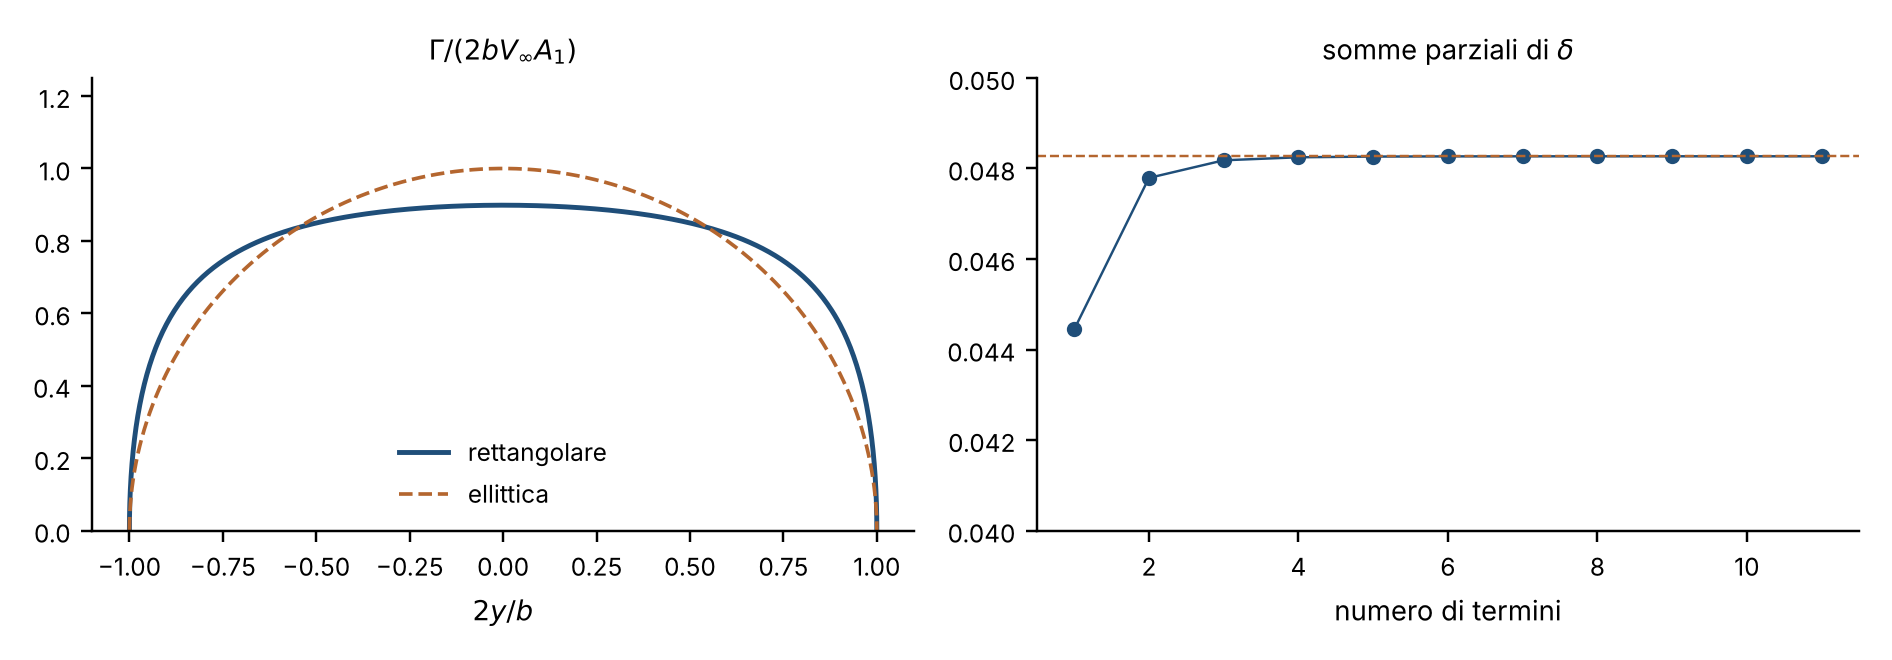
\includegraphics[width=\textwidth]{figure/resistenza_indotta.png}
\caption{A sinistra: la distribuzione di circolazione lungo l'apertura di un'ala
rettangolare con $AR=6$ (blu), confrontata con la distribuzione ellittica con la stessa
portanza (tratteggio rame). A destra: le somme parziali $\delta_{N}$ della serie
$\delta=\sum n(A_{n}/A_{1})^{2}$, crescenti e rapidamente convergenti, come deve accadere per
una serie convergente a termini non negativi (\texttt{python/fig\_resistenza\_indotta.py}).}
\label{fig:resistenza-indotta}
\end{figure}

\subsection{Approfondimento: prodotti infiniti e il prodotto di Wallis}
\label{subsec:prodotti-infiniti}

Come una serie è il limite delle somme dei suoi primi $n$ termini, così un \emph{prodotto
infinito} è il limite dei prodotti dei suoi primi $n$ fattori. Lo studio dei prodotti
infiniti si riconduce a quello delle serie, e conduce a una delle più antiche formule
per $\pi$.

\begin{definizione}[Prodotto infinito]\label{def:prodotto-infinito}
\index{prodotto infinito}
Sia $b_{k}>0$ per ogni $k\in\N$, e sia $p_{n}=b_{1}b_{2}\cdots b_{n}=\prod_{k=1}^{n}b_{k}$ il \emph{prodotto
parziale} $n$-esimo. Il prodotto infinito $\prod_{k=1}^{\infty}b_{k}$ si dice \emph{convergente} se
$p_{n}$ ha limite $P$ finito e \emph{positivo}, e allora si scrive $\prod_{k=1}^{\infty}b_{k}=P$; si
dice \emph{divergente} se $p_{n}\to+\infty$ oppure $p_{n}\to0$.
\end{definizione}

L'esclusione del limite $0$ è naturale. Passando ai logaritmi,
$\log p_{n}=\sum_{k=1}^{n}\log b_{k}$: se la serie $\sum\log b_{k}$ ha somma $L\in\R$, per la continuità
dell'esponenziale $p_{n}=e^{\log p_{n}}\to e^{L}>0$; viceversa, se $p_{n}\to P>0$, per la continuità del
logaritmo $\log p_{n}\to\log P$. Dunque \emph{il prodotto converge se e solo se converge la
serie dei logaritmi dei fattori}, e il caso $p_{n}\to0$ corrisponde a $\sum\log b_{k}=-\infty$. Come
per le serie, inoltre, se il prodotto converge i fattori $b_{n}=\frac{p_{n}}{p_{n-1}}$ tendono a
$\frac PP=1$: conviene scriverli nella forma $b_{k}=1+a_{k}$, con $a_{k}\to0$.

\begin{teorema}[Prodotti a fattori non minori di uno]\label{teo:prodotti-infiniti}
Sia $a_{k}\ge0$ per ogni $k$. Il prodotto $\prod_{k=1}^{\infty}(1+a_{k})$ converge se e solo se
converge la serie $\sum_{k=1}^{\infty}a_{k}$; altrimenti diverge a $+\infty$. Inoltre, dette $s_{n}$ e
$p_{n}$ le somme e i prodotti parziali,
\begin{equation}\label{eq:prodotti-stime}
  1+s_{n}\le p_{n}\le e^{s_{n}} \qquad\perogni n\in\N .
\end{equation}
\end{teorema}

\begin{schema}
\Ipotesi{$a_{k}\ge0$ per ogni $k$; \ $s_{n}=\sum_{k=1}^{n}a_{k}$, \ $p_{n}=\prod_{k=1}^{n}(1+a_{k})$.}
\Tesi{$1+s_{n}\le p_{n}\le e^{s_{n}}$; \ $\prod(1+a_{k})$ converge $\sse$ $\sum a_{k}<+\infty$; \
altrimenti $p_{n}\to+\infty$.}
\end{schema}

\begin{strategia}
Sviluppando il prodotto $(1+a_{1})\cdots(1+a_{n})$ si ottengono il termine $1$, tutti gli $a_{k}$ e
i loro prodotti, che sono non negativi: quindi $p_{n}\ge1+s_{n}$. La disuguaglianza
$1+x\le e^{x}$, applicata a ogni fattore, dà $p_{n}\le e^{a_{1}}\cdots e^{a_{n}}=e^{s_{n}}$. Le successioni $s_{n}$
e $p_{n}$ sono crescenti, e le due stime dicono che l'una è limitata se e solo se lo è
l'altra.
\end{strategia}

\begin{dimostrazione}
La prima delle \eqref{eq:prodotti-stime} si dimostra per induzione. Per $n=1$,
$p_{1}=1+a_{1}=1+s_{1}$. Se $p_{n}\ge1+s_{n}$, moltiplicando per $1+a_{n+1}>0$,
\[
  \begin{aligned}
  p_{n+1}&=p_{n}(1+a_{n+1})\ge(1+s_{n})(1+a_{n+1})\\
  &=1+s_{n+1}+s_{n}a_{n+1}\ge1+s_{n+1} .
  \end{aligned}
\]
Per la seconda, la \eqref{eq:exp-log-disuguaglianze} dà $0<1+a_{k}\le e^{a_{k}}$ per ogni $k$, e
moltiplicando membro a membro queste disuguaglianze tra numeri positivi
$p_{n}\le e^{a_{1}}e^{a_{2}}\cdots e^{a_{n}}=e^{s_{n}}$. La successione $p_{n}$ è crescente, perché
$p_{n+1}=p_{n}(1+a_{n+1})\ge p_{n}$, e $p_{n}\ge1$; per il \cref{teo:monotone} ha limite $P\in[1,+\infty]$.
Se $\sum a_{k}=s<+\infty$, allora $p_{n}\le e^{s_{n}}\le e^{s}$ e $P\in[1,e^{s}]$ è finito e positivo: il
prodotto converge. Se invece $s_{n}\to+\infty$, da $p_{n}\ge1+s_{n}$ e dal
\cref{teo:confronto-infinito} segue $p_{n}\to+\infty$.
\end{dimostrazione}

\begin{esempio}\label{es:prodotti-infiniti}
\begin{enumerate}[label=(\alph*)]
  \item Il prodotto $\prod_{k=1}^{\infty}\bigl(1+\frac1k\bigr)$ diverge: i fattori $\frac{k+1}k$ si semplificano «a
  cannocchiale» e $p_{n}=\frac21\cdot\frac32\cdots\frac{n+1}n=n+1$. La seconda delle \eqref{eq:prodotti-stime}
  diventa $n+1\le e^{H_{n}}$, cioè $H_{n}\ge\log(n+1)$: è la stima \eqref{eq:armonica-log}, che
  ritroviamo così per una quarta via.
  \item Il prodotto $\prod_{k=1}^{\infty}\bigl(1+\frac1{k^{2}}\bigr)$ converge, perché $\sum\frac1{k^{2}}$ converge, e per le
  \eqref{eq:prodotti-stime} il suo valore è compreso tra $1+\frac{\pi^{2}}6\approx2{,}64$ e
  $e^{\pi^{2}/6}\approx5{,}18$. (Il valore esatto è $\frac{e^{\pi}-e^{-\pi}}{2\pi}\approx3{,}68$.)
\end{enumerate}
\end{esempio}

Il prodotto infinito più celebre è quello di Wallis. I suoi fattori sono
$\frac{(2k)^{2}}{(2k-1)(2k+1)}=\frac{4k^{2}}{4k^{2}-1}=1+\frac1{4k^{2}-1}$, e poiché
$\frac1{4k^{2}-1}=\frac12\bigl(\frac1{2k-1}-\frac1{2k+1}\bigr)$, la serie $\sum\frac1{4k^{2}-1}$ è telescopica e
converge, con somma $\frac12$ (\cref{prop:serie-telescopica}): per il
\cref{teo:prodotti-infiniti} il prodotto converge, a un valore compreso tra $\frac32$ e
$e^{1/2}$. Il valore esatto viene dal calcolo integrale.

\begin{teorema}[Prodotto di Wallis]\label{teo:wallis}\index{prodotto di Wallis}
\begin{equation}\label{eq:wallis}
  \frac\pi2=\prod_{k=1}^{\infty}\frac{(2k)^{2}}{(2k-1)(2k+1)}
  =\frac21\cdot\frac23\cdot\frac43\cdot\frac45\cdot\frac65\cdot\frac67\cdots
\end{equation}
\end{teorema}

\begin{schema}
\Ipotesi{$I_{n}=\int_{0}^{\pi/2}\sen^{n}x\,dx$, con la formula di riduzione $I_{n}=\frac{n-1}nI_{n-2}$
per $n\ge2$ (\cref{es:wallis}); \ $W_{m}=\prod_{k=1}^{m}\frac{(2k)^{2}}{(2k-1)(2k+1)}$.}
\Tesi{$W_{m}\to\frac\pi2$.}
\end{schema}

\begin{strategia}
Iterando la formula di riduzione a partire da $I_{0}=\frac\pi2$ e $I_{1}=1$, l'integrale di indice
pari $I_{2m}$ contiene il fattore $\frac\pi2$ e quello di indice dispari $I_{2m+1}$ no, e il loro
rapporto risulta proprio $\frac\pi{2W_{m}}$. D'altra parte, poiché $0\le\sen x\le1$, le potenze
di $\sen x$ decrescono al crescere dell'esponente, e così i loro integrali:
$I_{2m+1}\le I_{2m}\le I_{2m-1}$. Questa catena intrappola il rapporto tra $1$ e $\frac{2m+1}{2m}$, che
tende a $1$, e il teorema dei carabinieri conclude.
\end{strategia}

\begin{dimostrazione}
Applicando $m$ volte la formula di riduzione (formalmente, per induzione su $m$),
\[
  I_{2m}=\frac{2m-1}{2m}\cdot\frac{2m-3}{2m-2}\cdots\frac12\cdot\frac\pi2 ,\qquad
  I_{2m+1}=\frac{2m}{2m+1}\cdot\frac{2m-2}{2m-1}\cdots\frac23\cdot1 .
\]
In particolare $I_{2m+1}>0$, e dividendo
\[
  \frac{I_{2m}}{I_{2m+1}}=\frac\pi2\prod_{k=1}^{m}\frac{2k-1}{2k}\cdot\prod_{k=1}^{m}\frac{2k+1}{2k}
  =\frac\pi2\prod_{k=1}^{m}\frac{(2k-1)(2k+1)}{(2k)^{2}}=\frac\pi{2W_{m}} .
\]
Per $x\in[0,\frac\pi2]$ si ha $0\le\sen x\le1$, e quindi
$\sen^{2m+1}x\le\sen^{2m}x\le\sen^{2m-1}x$; per il confronto tra integrali
(\cref{teo:confronto-integrali}), $I_{2m+1}\le I_{2m}\le I_{2m-1}$. Dividendo per $I_{2m+1}$ e usando la
formula di riduzione con $n=2m+1$, cioè $I_{2m-1}=\frac{2m+1}{2m}I_{2m+1}$, si ottiene
\[
  1\le\frac\pi{2W_{m}}\le\frac{2m+1}{2m}=1+\frac1{2m} \qquad\perogni m\in\N .
\]
Per il teorema dei carabinieri (\cref{teo:carabinieri}) $\frac\pi{2W_{m}}\to1$, e dunque
$W_{m}\to\frac\pi2$ (\cref{teo:operazioni-limiti}).
\end{dimostrazione}

L'ultima catena di disuguaglianze dice anche che
$0\le\frac\pi2-W_{m}\le\frac\pi2\bigl(1-\frac{2m}{2m+1}\bigr)=\frac\pi{2(2m+1)}$: l'errore è dell'ordine di $\frac1m$,
e la convergenza è lentissima. Il programma che segue mostra che ogni volta che il
numero dei fattori si moltiplica per dieci si guadagna una sola cifra esatta: il
prodotto $m\bigl(\frac\pi2-W_{m}\bigr)$ si stabilizza attorno a $\frac\pi8\approx0{,}3927$, cioè
$\frac\pi2-W_{m}\approx\frac\pi{8m}$, in accordo con la maggiorazione $\frac\pi{2(2m+1)}\approx\frac\pi{4m}$. Il
prodotto di Wallis non è dunque un metodo per calcolare $\pi$, ma un ponte tra il mondo
discreto dei prodotti di numeri interi e quello continuo degli integrali, che ritorna
nel calcolo delle probabilità e nella formula di Stirling per $n!$.

\needspace{14\baselineskip}
\begin{python}[La lenta convergenza del prodotto di Wallis]
import math

W = 1.0                                   # prodotto parziale W_m
for m in range(1, 10**6 + 1):
    W *= 4 * m * m / (4 * m * m - 1)
    if m in (10, 100, 1000, 10**4, 10**5, 10**6):
        err = math.pi / 2 - W
        print(f"m = {m:>7}: W_m = {W:.9f}  errore = {err:.2e}"
              f"  m*errore = {m * err:.5f}")
print(f"pi/2 = {math.pi / 2:.9f},  pi/8 = {math.pi / 8:.5f}")
\end{python}
\begin{risultato}
m =      10: W_m = 1.533851903  errore = 3.69e-02  m*errore = 0.36944
m =     100: W_m = 1.566893745  errore = 3.90e-03  m*errore = 0.39026
m =    1000: W_m = 1.570403873  errore = 3.92e-04  m*errore = 0.39245
m =   10000: W_m = 1.570757059  errore = 3.93e-05  m*errore = 0.39267
m =  100000: W_m = 1.570792400  errore = 3.93e-06  m*errore = 0.39270
m = 1000000: W_m = 1.570795934  errore = 3.93e-07  m*errore = 0.39270
pi/2 = 1.570796327,  pi/8 = 0.39270
\end{risultato}

\begin{notastorica}[Viète, Wallis, Brouncker, Newton]
Il primo prodotto infinito della storia è di François Viète (1593), che ottenne $\frac2\pi$
come prodotto di radici quadrate annidate studiando i poligoni regolari inscritti nel
cerchio. Il prodotto \eqref{eq:wallis} fu trovato da John Wallis, professore di geometria a
Oxford, nell'\emph{Arithmetica infinitorum} (1656), cercando l'area del quarto di cerchio,
cioè $\int_{0}^{1}\sqrt{1-x^{2}}\,dx=\frac\pi4$. Wallis sapeva calcolare gli integrali di $(1-x^{2})^{n}$ per
$n$ intero e ne «interpolò» il valore per $n=\frac12$, supponendo che la regolarità osservata
continuasse: un procedimento audace e senza dimostrazione, che il nostro
\cref{teo:wallis} giustifica a posteriori. Lord William Brouncker, futuro primo
presidente della Royal Society, trasformò il risultato in una frazione continua per
$\frac4\pi$, pubblicata nella stessa opera. Nell'inverno 1664--65 il giovane Isaac Newton
studiò l'\emph{Arithmetica infinitorum} e, applicando l'interpolazione di Wallis agli
integrali di $(1-t^{2})^{n}$ tra $0$ e un estremo variabile $x$, scoprì la serie binomiale
per esponenti frazionari (nota storica del \S\ref{sec:serie-taylor}). Circa ottant'anni
dopo il prodotto ricomparve come caso particolare di una scoperta di Eulero, la
scrittura del seno come prodotto infinito,
$\sen x=x\prod_{k=1}^{\infty}\bigl(1-\frac{x^{2}}{k^{2}\pi^{2}}\bigr)$, con cui nel 1734 egli ricavò la somma
$\frac{\pi^{2}}6$: con $x=\frac\pi2$ se ne ottiene proprio il prodotto di Wallis.
\end{notastorica}
